\documentclass[a4paper]{article}

\usepackage{geometry}
\usepackage{float}
\usepackage{amsmath, amssymb}
\usepackage{titlesec}
\usepackage{graphicx}
\usepackage{subfigure}
\usepackage{color}
\usepackage[hidelinks]{hyperref}
\usepackage[numbers,square,super,sort&compress]{natbib}
\usepackage{enumitem}
\usepackage{siunitx}
\usepackage{listings}
\usepackage{cprotect}
\usepackage{subfig}

\setlength{\parskip}{0.25cm}
\setlength{\parindent}{0cm}

\lstset{language=Python, showstringspaces=false, basicstyle=\small,
  numbers=left, numberstyle=\tiny, numberfirstline=false, breaklines=false,
  stepnumber=1, tabsize=4, 
  commentstyle=\ttfamily, identifierstyle=\ttfamily,
  stringstyle=\itshape}

\title{\vspace{-15mm}\fontsize{24pt}{10pt}\selectfont\textbf{Vitalik's Place\footnote{Disclaimer: This project is not associated to nor endorsed by Vitalik Buterin. The name is chosen in the style of Satoshi's Place created by LightningK0ala.}}}
\author{
\large
{\textsc{Hilobrain}}}

\begin{document}
\maketitle{}

\setcounter{tocdepth}{2}
\tableofcontents%

\newppage%

\section{Introduction}
Vitalik's Place is a massive online shared canvas on the Ethereum blockchain consisting of 1 million pixels, with some of them holding Ethereum. When you are lucky and draw the right pixel, you earn the jackpot that consists of a certain amount of ether! The more pixels are drawn over time, the bigger the jackpot gets! The project is heavily inspired by Reddit's Place, the Million Dollar Webpage and especially Satoshi's Place. This documentation is written to explain all components of the system for those interested. Although all being publicly verifiable on the Ethereum blockchain, this documentation also explains, justifies and analyses the mechanisms that are involved in the random process of picking winners and prizes.

\section{System Overview}
The system overview is devided into two parts; the front end and the back end. The back end is then subdevided into the smart contract that operates on the Ethereum blockchain and the local server hosted by myself to ensure fast loading times of the canvas. The diagram below shows how all the individual parts are connected.

\begin{figure}[H]
    \centering
    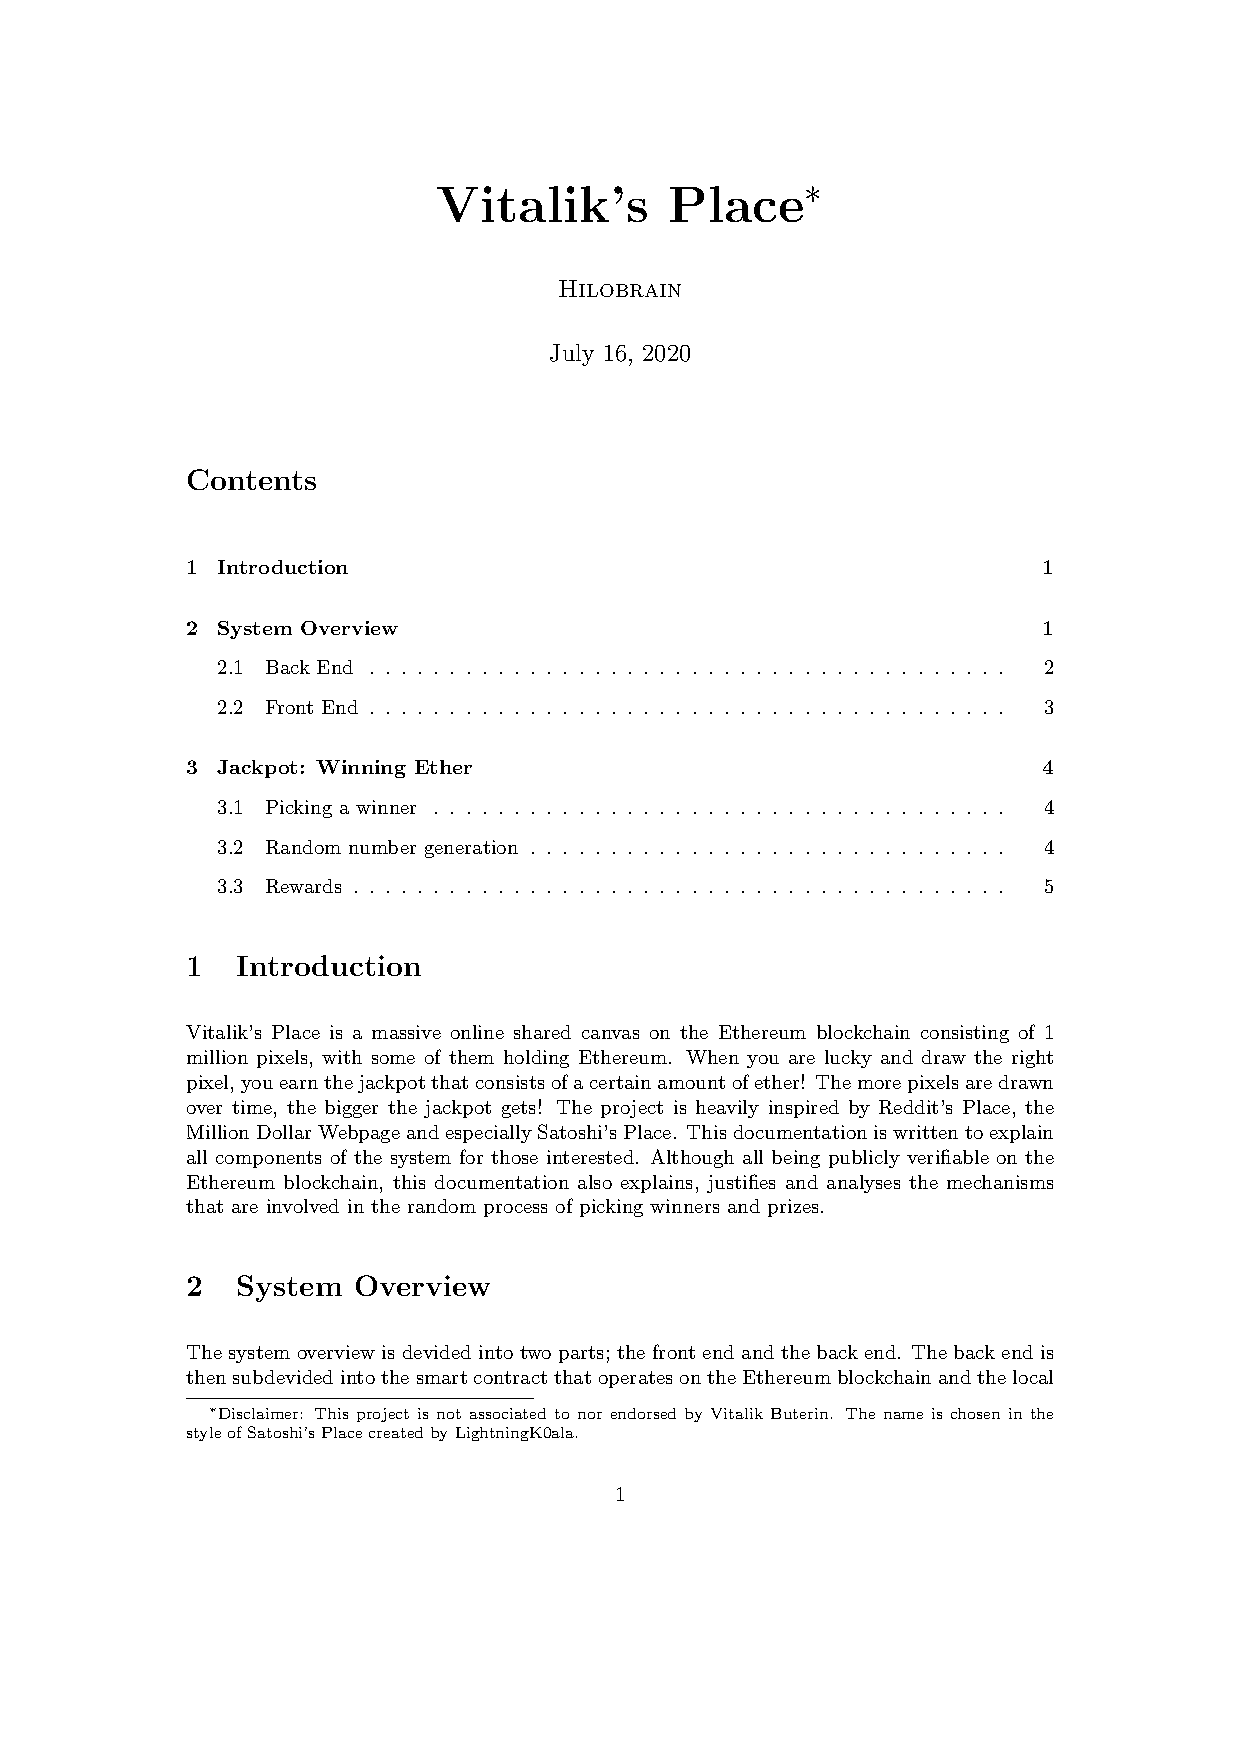
\includegraphics[width=\textwidth]{Vitaliks_Place.pdf}
    \caption{A schematic overview of the parts making up the whole system. The arrows show the flow of information/interactions, e.g. the front end pulls information from the smart contract and the Github canvas and gets input from you, the user. The local server pulls information from the smart contract through Infura.}
    \label{fig:1}
\end{figure}

\subsection{Back End}

\subsubsection{Smart Contract}
The core of Vitalik's Place is the smart contract that is ``live'' on the Ethereum blockchain\footnote{The code can be verified here: \url{URL OF SMART CONTRACT ETHERSCAN HERE}}. This smart contract keeps track of the ownership of all the pixels, keeps a history of painting events, calculates whether one wins a prize (in the form of Ethereum) or not.
\paragraph{Drawing pixels:}
The main function of the smart contract is the \lstinline{draw_pixels} function, allowing users to draw multiple pixels at once. The function requires three arrays: the x-positions of the pixels, the y-positions and the indexed colors. These arrays must be of equal length and the transaction value (the cost of the pixels) must be greater or equal to the amount of pixels drawn times the price per pixel. \\
When these requirements are satisfied, the pixels get added to the eternal memory in the form of a big array containing pixels. The smart contract then determines whether you win the jackpot or not, see the section Jackpot: Winning Ether for information about this process. Finally, an event containing information about the pixels drawn is emitted such that listening clients can update their canvasses accordingly.
\paragraph{Pixel memory:} The contract keeps track of the position and color of all pixels ever to be painted on the contract, also pixels that get drawn over by other users. To do this efficiently, a struct called \lstinline{Pixel} is created. This object has three properties: a x-coordinate, y-coordinate and a indexed color. These objects get stored in an array making up the whole canvas. To save on gas costs indexed colors are used; these are single digit numbers representing pre-determined colors. This way, we only have to store a single digit number instead of a hexadecimal string or RGBA values. As we have a predetermined palette for users to choose from (otherwise the canvas would get ugly very fast...) the limited amount of colors is not a problem.

\subsubsection{Local Server}
A dedicated server hosts a program that constantly listens for paint events from the smart contract and keeps track of this on a local copy. Once a user has succesfully painted one (or more) pixel(s) on the canvas the bot updates its local copy and uploads a base64 encoded version of the canvas to the GitHub repository (at: \url{https://github.com/Hilobrain/Vitaliks-Place/blob/master/canvas/canvas_base.txt}). This file is then used by the front end once the user opens up the website. This way, the front end does not have to make any calls to the smart contract to get the current canvas status, ensuring near-instant loading times.

\subsection{Front End}
The front end runs on my personal github pages (\url{https://hilobrain.github.io}). This allows the website to be run without having any server costs or maintenance. The front end interacts with the smart contract through web3 injected by Metamask. The website can also be viewed without Metamask but then (obviously) the smart contract interaction-features like drawing pixels, the jackpot counter on the top right, etc., won't work. \\
On the openening of the website, the front end detects injected web3 by Metamask and asks the user to connect in order to proceed. When succesful, the network to which the wallet is connected is checked such that the user is connected to the main Ethereum network instead of other testnetworks. When the initialization phase has succeeded, the user is good to go and can then interact with the smart contract through the front-end. \\
The front end automatically subscribes to two events from the smart contract in the background: the \lstinline{winner} event (emitted when someone has won the jackpot) and the \lstinline{canvas_updated} event (emitted when new pixels have been drawn on the canvas). These events are used to give the user feedback on what happens on the front end. This means that when someone else draws pixels and the transaction is confirmed and you are on the website too, you see the pixels being drawn live! This is the power of smart contract events in combination with web3! This also allows the front end to update necessary variables like the jackpot value when new pixels are drawn to the canvas. This way, what you see is what you get.
On the loading of the website another important component of the system comes in to play; the local server that updates the Github for the front end to get the current state of the canvas from. To get the full state of the canvas on the loading of the website, it has to get all information of all pixels ever to be drawn, in the right order. This would take increasingly more time as more pixels get drawn to the canvas and would result in insanely (think minutes/hours) long loading times. To work around this, I've built a local server that watches the smart contract 24/7 and keeps track of the current state of the canvas in local files, as explained under the section Local Server. The front end can then simply load the base64-encoded canvas from the Github page ensuring near-instant loading times. Should the local server go down for some reason, the front end might not reflect the actual state of the canvas anymore. However, this does not mean the pixels are gone or the contract is broken. The local server will be fired up as soon as possible which will immediately update the canvas back to its newest state. The actual state can also be verified 24/7 using the transactions to the smart contract. \\
This also introduces a minor disadvantage of the system: when a user draws pixels and reloads the website after transaction confirmation, the pixels might not show up immediately as the Github page needs some time to update the contents of the file. The front end then uses the old base64 encoded image and thus the new drawing won't show. It takes a maximum of 5 minutes (usually less than 1 minute) for it to be updated. This means that when a user draws some pixels, there is a small window (of said time) in which other users that load the website won't see the new drawings. As this window is particularly small and it isn't a fast-pace interactive website, this is considered to not be a problem.

\section{Jackpot: Winning Ether}
In this section the methodology of chosing a winner is explained as well as the security considerations. 

\subsection{Picking a winner}
When a user draws pixels on the canvas, he/she might be lucky and get ether if he/she drew (on of) the lucky pixel(s)! Everytime a user paints a set of pixels, the amount of pixels drawn is stored. Naturally, the more pixels a user draws, the bigger the chance of winning the jackpot. A variable in the smart contract called \lstinline{win_chance} determines how many lucky pixels there are on the canvas, e.g. when \lstinline{win_chance = 999999} there is exactly one lucky pixel on the canvas. The smart contract picks a random number from 0 up to and including \lstinline{win_chance}. When this number is lower than the amount of pixels drawn by the user he/she wins the jackpot. The costs of the pixels drawn in the transaction that caused the user to win the jackpot are included in the reward.

\subsection{Random number generation}
Creating a random number can be quite tricky for smart contracts to do. To create a random number the following variables are hashed together as a encoded packed using keccak256: \lstinline{block.timestamp}, \lstinline{block.difficulty}, \lstinline{block.number} and the amount of pixels drawn. This hash is then converted to uint256 resulting in a random number. \\
Some of the data that is hashed to create the random number can be \emph{influenced} by the miners on the Ethereum network to a certain degree: the block timestamp and to a certain extend the block number and block difficulty. Note that influenced does not mean that the miners are entirely free to choose these parameters as the Ethereum network does not allow them to do so. The amount of pixels drawn can obviously also be entirely determined by the user itself. However, for a hacker to confidently create random numbers to his/her likings, he/she has to have significant control over the miners, which costs a lot of money. I expect that the costs of controlling this outgrow the potential reward by orders of magnitude making this attack not feasible. There are also many other higher-profile targets out there that will draw the attention would one be able to influence these parameters confidently.

\subsection{Rewards}
When a user is lucky and wins the jackpot, the ether is automatically send to the user and he/she is congratulated with a nice notification. The amount that is available to win is always exactly half of the balance of the contract. The balance of the contract increases as users pay for pixels. This means that the more pixels are drawn to the canvas, the bigger the prize. The bigger the prize, the more users would give it a try. This creates a run-away effect incentivizing drawing pixels while e.g. allowing individuals or companies to relatively cheaply place ads. In figure \ref{fig:2} a plot is made for the optimum strategy for different contract balances (which is expected to grow over time).

\begin{figure}[H]%
    \centering
    \includegraphics[width=0.75\textwidth]{optimum_strategy.pdf} %
     \caption{The optimum strategy for a user for certain contract balances. On the horizontal axis the fraction of the canvas to draw is given. The vertical axis represents the \emph{expected} profit, i.e. the profit times the chance of actually winning the jackpot. The most optimal amount of pixels to draw is indicated with a cross. As can be seen in the figure, when there is 1000 ethereum in the contract, it is most optimal to draw 25\% of the canvas. The numbers for the contract balances here are chosen merely as a demonstration.}%
    \label{fig:2}%
\end{figure}

The expected profit is calculated by taking the potential profit from the jackpot when a user wins and multiplying that with the chance of actually winning the jackpot. This means that e.g. when the contract has 1000 ether as a balance, the jackpot is 500 ether. And thus, as can be seen in the figure, it is most optimal to draw 25\% of the canvas (250000 pixels). The potential profit is then $500 - 250000 \cdot 0.01 = 250$ ether. Now, since you have a chance of 0.25 of winning the jackpot when drawing 25\% of the canvas, the expected profit is then $250 * 0.25 = 62.5$ ether, as can also be seen in the figure in the purple curve. \\
This means that the more pixels are drawn, the more pixels should be drawn for the optimal strategy of winning the ether that is present in the smart contract.

\end{document}
